\section[Swing komponenter]{Tilpassede \emph{Swing} komponenter} \label{sec:swing}
I programmet er det brukt flere spesialtipassede komponenter arvet fra swing klassen med f.eks for størrelse, brukerinteraksjon eller andre tilpassninger. Komponentene er plassert i pakke \texttt{view} og \texttt{view.register}. I dette avsnittet beskrives spesielt tilpassede eller komponenter som har spesifikk betydning for programmet.

\subsection{\texttt{AbstractPanel.java}} \label{subsec:AbstractPanel}
Abstract panel som arver \texttt{JPanel} er klassen som ligger til grunn til alle paneler som er i bruk i programmet. Klassen har to konstruktører og har som regel følgende oppgaver:
\begin{itemize}
\item Setter størrelse (dimensjon) på panelen.
\item Setter bakgrunnfarve på panelen fra gn global static konstant. Dette gjør at farve på all brukegrensesnitt i programmet kan enkelt endres.
\item Sette en \texttt{titleBorder} rundt komponenten fra parameter i konstruktøren. Avhengig av hvilken kontsruktør som brukes.
\end{itemize}
Dimensjonen settes gjennom å kalle opp metoden \texttt{setPrefferedSize(Dim dim)} som brukes ettersom slik tilnærming gjør at størrelse på panelen blir "<respektert"> av valgt layout manager (dette gjelder ikek altid dersom \texttt{setSize()} brukes.




\subsection{\texttt{MainPanel.java}}
MainPanel er klassen som arver AbstractPanel og setter oppbåde megler og annonse panelen, se eksempel \ref{kode:main_panel}. Arv fra superklassen består gjennom at man kaller opp en tom konstruktør i superklassen som setter opp bakgrunnfarve. Deretter blir det satt opp en enkel gridlayout som består av en celle. Cellen splittes opp og i den plasseres to \texttt{JPanel} og en \texttt{JTabbedPane} som legger til panel for annonse og megler. Klassen \texttt{MainPanel} blir deretter initilisert fra \texttt{StartGUI.java} ved oppstart av programmet. 


\begin{lstlisting}[caption=Kontruktør i \texttt{MainPanel.java}, label=kode:main_panel]
    public MainPanel(AbstraktArkfane megler, AbstraktArkfane annonse){
        setLayout( new GridLayout( 1, 1)) ;
        this.megler = (JPanel) megler;
        this.annonse = (JPanel) annonse;
        
        arkfaner = new JTabbedPane(JTabbedPane.TOP);
        
        //Legger til tab og kobler med panelet.
        
        arkfaner.addTab("Megler  ", Ikoner.MEGLER, this.megler);
        arkfaner.addTab("Annonser  ", Ikoner.ANNONSER, this.annonse);
        
        arkfaner.setSelectedIndex(1);
        arkfaner.setToolTipTextAt(0, "Administrering av boliger, søknader mm.");
        arkfaner.setToolTipTextAt(1, "Finn tilgjengelige boliger, send inn søknader mm.");
        
        add(arkfaner);
    }
\end{lstlisting}



\subsection{\texttt{AbstraktArkfane.java}}
Abstract klasse som arver \texttt{AbstractPanel}. Klassen som arver den får et oppsett av paneler. Hvilket oppsett av paneler som blir oprettet er avhengig av hilken parameter som blir sendt inn i konstruktøren se eksempel +ref{kode:arkfane}. Hvilke type av arkfane som skal bli oprettet bestemmes a streg parametern som blir sendt inn til konstruktøren. Klassen arves av to klasser: \texttt{ArkfaneMegler.java} og \texttt{ArkfaneAnnonse.java} hvilke setter begge faner i programmet. 

\begin{lstlisting}[caption=Konstruktør til \texttt{AbstraktArkfane}. label=kode:arkfane]
    public AbstraktArkfane(String valgtToppanel) {
        setLayout(new BorderLayout());
        setVisible(true);
        
        bunnpanel = new BunnPanel(VinduStorrelse.BUNNPANEL.getHEIGHT(), 
                VinduStorrelse.BUNNPANEL.getWIDTH());
        venstrepanel = new VenstrePanel("Liste",VinduStorrelse.VENSTREPANEL.getHEIGHT(), 
                VinduStorrelse.VENSTREPANEL.getWIDTH());
        senterpanel = new SenterPanel("Visning",VinduStorrelse.SENTERPANEL.getHEIGHT(), 
                VinduStorrelse.SENTERPANEL.getWIDTH());

        if (valgtToppanel.equals("megler")) {
            toppanel = new TopPanelMegler("Søk",VinduStorrelse.TOPPANEL.getHEIGHT(), 
                    VinduStorrelse.TOPPANEL.getWIDTH());
            add(toppanel, BorderLayout.NORTH);
        } else{
            toppanel = new TopPanelAnnonse("Søk",VinduStorrelse.TOPPANEL.getHEIGHT(), 
                    VinduStorrelse.TOPPANEL.getWIDTH());
            add(toppanel, BorderLayout.NORTH);
        }
        add(venstrepanel, BorderLayout.WEST);
        add(senterpanel, BorderLayout.CENTER);
        add(bunnpanel, BorderLayout.SOUTH);
    }
\end{lstlisting}



Som vi kan se i koden AbstraktArkfane setter opp komponenter som inngår i de to visningsfanene fordelt på \texttt{Annonse} eller \texttt{Megler}. Klassen innholder også en layoutmanager som setter opp alle disse komponentene med rettninger: NORTH, WEST, CENTER og SOUTH. Resultatet av dette presenteres i figur \ref{fig:asbtarkfane} der alle de forskjellige delen i som settes opp i klassen er satt opp. Klassen består også av et fleretall get metoder som kan brukes til å returnere hele paneler til kontrollere i MVC strukturen. Klassen blir arvet av følgende sub-klasser: (1) \texttt{ArkafaneAnnonse.java} og (2) \texttt{ArkfaneMegler.java}. hver enkel av disse subklassser kaller opp kontruktøren i superkalssen \texttt{AbstraktArkfane} som initialiserer layouten og setter opp riktige paneler.




\begin{figure}[ht]
 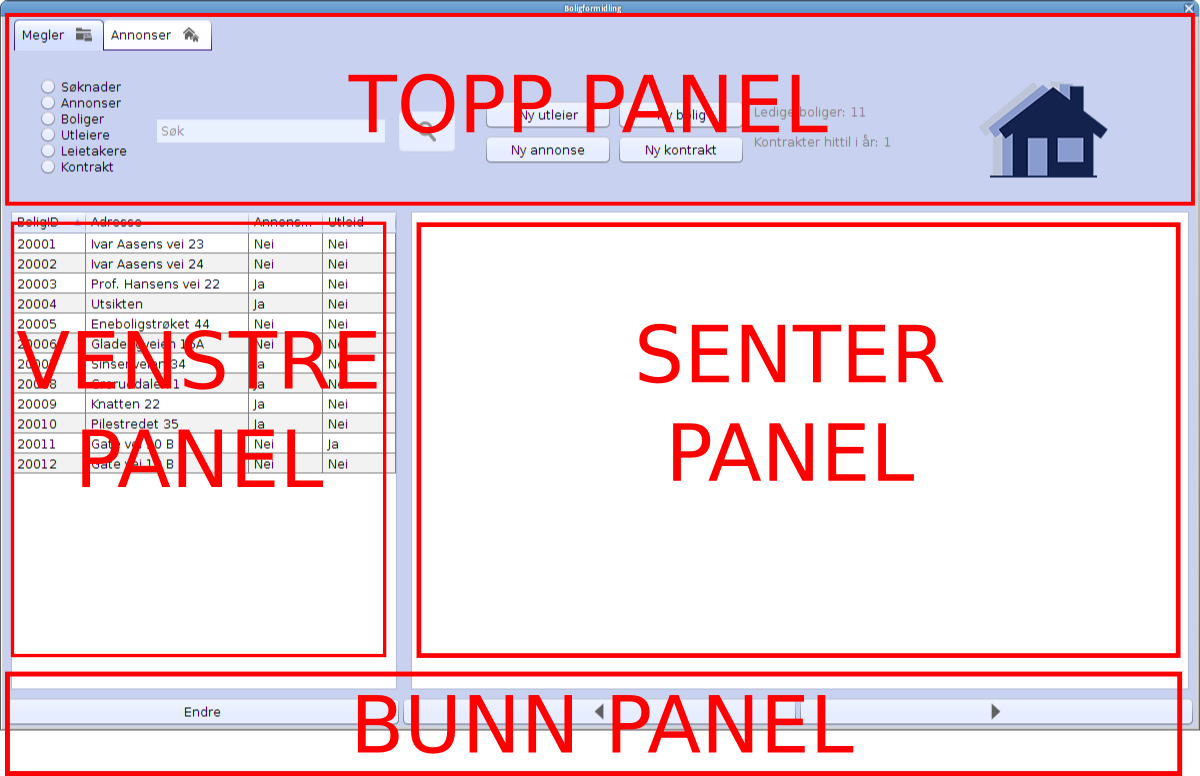
\includegraphics[width=\textwidth,height=\textheight,keepaspectratio]{./img/produktdokumentasjon/swing_componenter/AbstraktArkfane.png}
 \caption{Fordeling mellom komponenter i AbstraktArkfane}
 \label{fig:asbtarkfane}
\end{figure}



\subsection{\texttt{MeglerPanel.java}} \label{subsec:meglerpanel}
Meglerpanelen (figur \ref{fig:megler_panel}) er kontrollert fra \texttt{ControllerToppPanelMegler.java}, komponentene i den topppanelen blir aktivert og deaktivert avhengig av hvilket register eller funkjson brukeren har valgt for tilfellt. Eksepel på dette er når brukeren for første ette programstart går inn til panelen vil søkefeltet være deaktivert frem til riktig radiobutton velges for det register som man ønsker å søke i. Liknende funkjsonalitet er lagt inn dersom man f.eks. ønsker å registrere en ny bolig. En bolig kan kun registreres på en "<person"> som i dette fall kan være en eier eller en representant. For at man ikke skal ha mulighet til å registrere en bolig uten en eier er det alerede sperret på GUI lager slik at brukeren må markere en alerede registrert eier i eierlisten og deretter klikke på \texttt{Ny bolig} knappen. Så lenge ingen person er marker i tabellen vil knappen forbli deaktivert. Analogt til den fun ksjonaliteten er det lagt til liknende begrensninger for oprettelse an en ny annonse, da det må markeres et boligobjekt i tabellen for å få lov å oprette en ny annonse. Deretter for å oprette et nytt kontrakt må det ha ankommet en forespørsel til megleren som velger først å markerer forespørselen for hvilken kontrakt skal oprettes. 

\begin{figure}[ht]
 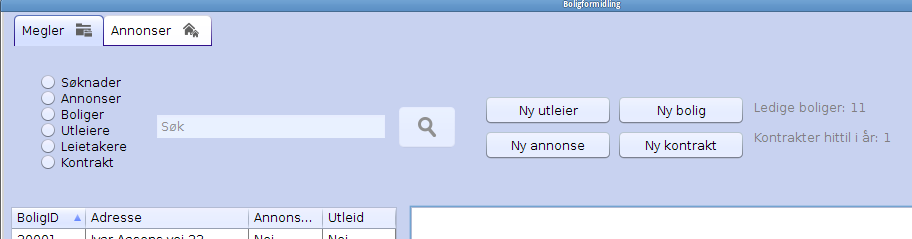
\includegraphics[width=\textwidth,height=\textheight,keepaspectratio]{./img/produktdokumentasjon/swing_componenter/megler_panel.png}
 \caption{GUI komponenter i meglerpanel}
 \label{fig:megler_panel}
\end{figure}




\subsection{\texttt{CustomSubPanel.java}}
Klassen arver de abstrakte klassen \texttt{AbstractPanel.java} (avsnitt \ref{subsec:AbstractPanel}). brukes til å sette opp indre paneler i alle registreringsvinduer som f.eks. registrering av nye boliger, utleier osv. Klassen er utstyrt med flere konstrutører som kan ta kombinasjoner av titel, dimensjoner og layout manager. Slik valgfrihet gir at panelen kan initialisere på mange forskjellige måter og enkel kan benyttes utefre forskjellige krav som kan stilles på slik panel i brukegrensesnittet. Panelen innholder også en metode for å ta imot en lytter (\texttt{ActionListener}) for en enkel og rask implementering i sammmen med en kontroller klasse etter MVC arkitektur.








\subsection{\texttt{CustomJTextField.java}}
\texttt{CustomJTextFiled} arver \texttt{AbstractPanel} og dermed innholder samme konstruktør som denne panelen hvilken setter feltets dimensjoner. Slik løsning medfører også at hvert tekstfelt er plasser i en egen \texttt{JPanel}\footnote{arves av \texttt{AbstractPanel}}.
Tekstfeltet er spesiltipasset slik at en den innholder en indre label som kan for eksempel brukes til å sette en mal på hva brukeren skal skrive inn i tekstfeltet. Eksempelvis kan dette være forventet antall sifferer i et telefon- eller personnummer, figur \ref{fig:custom1}. Feltet innholder også to lytter for \texttt{focusEvent} som initialiserer en regex etter en regex mønster som settes via feltets kontruktør. Regex mønster hentes via static konstant som passer et uttrykk som feltet skal brukes til (se avsnitt \ref{subsec:regextest}, side \pageref{subsec:regextest}). Etter at markøren flyttes ut fra feltet hvis da regex testen feilr blir feltet markert med rød farve som det vises i figur \ref{fig:custom2}.
Panelen overrider også de metoder som man ønsker at skal være tilgjengelige fra superklassen \texttt{JTextField} som er \texttt{getText()}, \texttt{setText()} og \texttt{setEnabled()}.

\begin{figure}[ht!]
\centering
\begin{subfigure}[b]{1\textwidth}
\centering


\includegraphics[scale=0.7]{./img/produktdokumentasjon/swing_componenter/1.png}
\caption{Inaktiv, indre label}
\label{fig:custom1}
\end{subfigure}
\quad

\begin{subfigure}[b]{1\textwidth}
\centering

\includegraphics[scale=0.7]{./img/produktdokumentasjon/swing_componenter/2.png}
\caption{Regex kontroll feilet}
\label{fig:custom2}
\end{subfigure}
\quad

\caption{Forsjellige tilstand av CustomJPane}\label{fig:customjpane}
\end{figure}



\subsection{\texttt{CustomJButton.java}}
Klassen arver \texttt{JButton} og består av totalt fem forskjellige kontruktører (se eksempel \ref{kode:customButton} som brukes til å sette opp en spesifikk knapp. Konstruktørene er diversifisert på en måte slik at det kan settes opp knapper med forskjellige størrelser, titler, ikoner eller også kombinasjoner av alle disse muligheter. 

\begin{lstlisting}[caption=De forskjellige konstruktørene i \texttt{CustomJButton}. ,label=kode:customButton]
public class CustomJButton extends JButton {

    private String navn;
    private Icon ikone;

    public CustomJButton(String navn) {
        this.navn = navn;
        setText(this.navn);
    }

    public CustomJButton(String navn, int bredde, int hoyde) {
        this.navn = navn;
        setText(this.navn);
        setPreferredSize(new Dimension(bredde, hoyde));
    }

    public CustomJButton(String navn, Icon ikone) {
        this.navn = navn;
        this.ikone = ikone;
        setText(this.navn);
        setIcon(this.ikone);
    }

    public CustomJButton(Icon ikone) {
        this.ikone = ikone;
        setIcon(this.ikone);
    }

    public CustomJButton(Icon ikone, int bredde, int hoyde) {
        this.ikone = ikone;
        setIcon(this.ikone);
        setPreferredSize(new Dimension(bredde, hoyde));
    }
}
\end{lstlisting}





\subsection{\texttt{ComboDatoVelger.java}}
Datovelger implementerer \texttt{CustomSubPanel} men hjelp av en egen layout manager. Klassen brukes med med hensikt å implemntere en datovelger som skal gjøre det mulig for å velge riktig dato uten å bruke regex hvilket i sin tur skal oppleves enklere for brukeren. Komponentene består av tre \texttt{JComboBox} som brukes for valg av år, måned og deretter dag. Velgeren er utstyrt med en egen lytter som setter riktig antall dager i den siste listen etter at brukeren har valgt år og måned (se figur \ref{fig:combo_datovelger}).
Klassen kan returnere valgt data etter int fordelt per år, måned og dag samt et \texttt{Calender} objekt dersom så ønkes. Dato kan også blir satt gjennom å oppkalle metoden \texttt{setDato(int ar,int mnd, int dag)} hvilket er en funkjson som brukes ved f.eks editering av de registrerte boligene. 


\begin{figure}[ht]
\center
 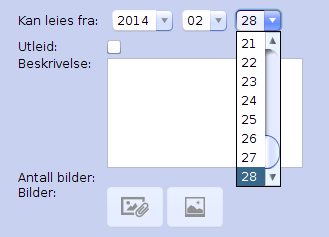
\includegraphics[scale=0.5]{./img/produktdokumentasjon/swing_componenter/combo_datovelger.png}
 \caption{\texttt{ComboDatoVelger.java} tilpasning av antall dager.}
 \label{fig:combo_datovelger}
\end{figure}

